\section{Problema 3: Guardando el tesoro}

\subsection{Introducción}

En medio del viaje, nuestros arqueólogos encuentran una sala llena de tesoros que desean llevar a su casa utilizando las mochilas con las que disponen. Deberán distribuir los objetos de manera lo suficientemente eficiente como para maximizar el valor total entre todas las mochilas sabiendo que cada una de estas tiene un tope de peso que pueden llevar.

Dicho formalmente, si tenemos un conjunto de $n$ objetos $O = \{(p_i,v_i) \quad | \quad 1 \leq i \leq n\}$ con peso $p_i$ y valor $v_i$ y $m$ mochilas con capacidad $K_j$, queremos encontrar distribuir los $o_i$ en cada mochila $M_j$ de manera tal de maximizar $\sum_{j = 0}^m\sum_{o_i \in M_j} v_i$ (es decir, la suma total del valor de cada mochila) sin exceder su capacidad de peso (Osea, $(\sum_{o_i \in M_j} p_i) \leq K_j$).

Este tipo de problema es conocido como Multiple Knapsack.

\subsection{Solución}

Antes de presentar la solución se aclara que, a diferencia de como se presenta en el enunciado, se tienen en cuenta a todos los tesoros como si fueran distintos. Es decir, por ejemplo, si hay 4 unidades de un mismo tesoro, se tienen en cuenta a cada uno como tesoros distintos de igual peso y valor.

Para solucionar el problema, se utilizó programación dinámica de la siguiente manera:

\begin{itemize}
\item Se empieza suponiendo que todas las mochilas tienen capacidad 0. Se van haciendo pruebas y se va aumentando en 1 el tamaño de cada una hasta llegar a la capacidad máxima original de todas las mochilas (en otras palabras, se prueba con todas las combinaciones de tamaños posibles)
\item Estas pruebas consisten en ver, dada una combinación de capacidades máximas, cuál es la combinación de objetos que genera el máximo valor sin superar la cota de ninguna mochila.
\item Para ver eso, se van probando los objetos uno por uno en cada mochila. Si el objeto $i$ entra en la mochila $j$, se consulta un valor previamente calculado, el cual es el resultante de hacer este mismo procedimiento con la misma configuración de mochilas, con la diferencia de que a la mochila $j$ se le resta el peso del objeto $i$. Si ese valor sumado al valor del objeto $i$ supera al que venía siendo el candidato a valor máximo, será reemplazado por este mismo.
\end{itemize}

Sobre el último ítem: lo que se hace cuando se consulta el resultado anteriormente calculado es tener en cuenta que hay un invariante en el algoritmo: todos los resultados anteriores son el valor óptimo calculado para la combinación de pesos máximos dada. Entonces, si se pregunta por una combinación en la cual el peso de una de las mochilas es menor, se tiene la seguridad de que eso ya fue calculado y es el mejor valor. Si el objeto con peso $p_i$ entra en la mochila $j$, se trata de encontrar cuál es la mejor combinación con el peso restante de la mochila $j$, dejando a las otras mochilas intactas y sin tener en cuenta al objeto $i$ para luego sumar $p_i$ a la mochila y $v_i$ al valor total. Si eso supera al candidato a máximo que había antes, entonces se vuelve el mejor candidato global y el mejor valor para la combinación actual de capacidades máximas de mochila. De lo contrario, se mantiene al mejor candidato global como estaba y al mismo tiempo pasa a ser el mejor valor para la combinación actual de mochilas.

A continuación se presenta el pseudo-código asociado al algoritmo que resuelve el problema:

\lstset{basicstyle=\large}
\begin{lstlisting}
input: mochilas : vector<int>,  objetos : vector<int>

mejorValor $\leftarrow$ crear un vector de $m+1$ dimensiones
int mejorValorGlobal
mejorCombinacion $\leftarrow$ vector de longitud $m$
para toda combinacion $p$ de pesos de mochilas $w_1 \ldots w_m$ (recorridas en un orden crecinte)
	int valorCandidato
	para todo $i$ desde $1$ hasta $n$
		valorAnterior  $\leftarrow$ $mejorValor[w_1][w_2]\ldots[w_m][i-1]$
		para todo $j$ desde $1$ hasta $m$
			si el objeto $i$ entra en la mochila con peso $w_j$
				valCandidato $\leftarrow$ $mejorValor[w_1]\ldots[w_{j-1}][w_j - p_i][w_{j+1}]\ldots[w_m][i-1]$
			sino
				valorCandidato $\leftarrow$ $-1$
			si valorAnterior < valorCandidato
				pongo el objeto en la mochila con peso $w_j$
				valorAnterior $\leftarrow$ valorCandidato
	si valorCandidato $>$ mejorValorGlobal
		mejorValorGlobal $\leftarrow$ valorCandidato
		mejorCombinacion $\leftarrow$ p

\end{lstlisting}

\subsubsection{Correctitud}

Para demostrar correctitud del agoritmo, se utiliza inducción doble en la cantidad de objetos y en las combinaciones de pesos parciales de mochilas. Para lo segundo, se define una relación de orden parcial bien fundada de la siguinte manera:

Dadas $m$ mochilas y dos vectores de pesos $p$ y $p'$ de dimensión $m$

$$p \leq p' \Leftrightarrow p_i \leq p'_i \quad \forall \quad 1 \leq i \leq m$$

También, existe un elemento mínimo $0_m$ que es el vector con ceros en todas sus coordenadas y cumple

$$0_m \leq p \quad \forall p$$

Una vez definida la relación de orden parcial, podemos pasar a la demostración:

\vspace{5mm}

{\Large\textbf{Mochilas: Caso base}}

\vspace{5mm}

Para esta instancia consideramos al menor elemento en nuestro orden de vectores: $0_m$.

\vspace{5mm}

{\large\textbf{Objetos: Caso base}}

\vspace{5mm}

Si tenemos el vector $0_m$ y $0$ objetos, el resultado es trivial ya que el valor máximo es $0$ y para cada mochila se introducen $0$ objetos.

\vspace{5mm}

{\large\textbf{Objetos: Paso inductivo}}

\vspace{5mm}

Para este caso, contamos con el vector $0_m$ y los $n$ primeros objetos. Si separamos alguno de ellos y miramos los $n$ restantes, por hipótesis inductiva, nuestro algoritmo devolverá el mejor valor para esa instancia. Si se mira el objeto $n + 1$, se puede ver que este no entra en ninguna mochila y por ende no se lo tiene en cuenta. Entonces, la solución para $n + 1$ objetos es la misma que para $n$.

\vspace{5mm}

{\Large\textbf{Mochilas: Paso inductivo}}

\vspace{5mm}

Para esta instancia, dado un vector de pesos $p$ cualquiera, queremos probar que el algoritmo resuelve el problema sabiendo que puede hacerlo para cualquier vector menor o igual a $p$.

\vspace{5mm}

{\large\textbf{Objetos: Caso base}}

\vspace{5mm}

Si tenemos el vector $p$ y $0$ objetos, el resultado vuelve a ser trivial y no se necesita utilizar la hipótesis inductiva ya que el valor máximo es $0$ y para cada mochila se introducen $0$ objetos.

\vspace{5mm}

{\large\textbf{Objetos: Paso inductivo}}

\vspace{5mm}

Para esta demostración, resulta importante entender las hipótesis con las que se cuenta:

\begin{itemize}
\item Para el vector $p$, el algoritmo sabe resolver todas las instancias del probema con $n$ objetos.
\item Para cualquier vector $p' \leq p$, el algoritmo sabe resolver todas las instancias del problema con $k$ objetos (donde $k$ es cualquier natural que podría ser mayor a $n$, aunque eso no se usa en esta demostración)
\end{itemize}

Entonces, dado el vector $p$ y $n + 1$ objetos, hay $m + 1$ opciones que conciernen al objeto $n + 1$-ésimo: o no se lo pone en ninguna mochila, o se lo pone en alguna de las $m$ mochilas. La opción que genere el valor máximo será la que solucione el problema.

Si no se lo incluye en ninguna mochila, se resuelve el problema para los $n$ primeros objetos y por hipótesis inductiva (primer ítem) el algoritmo brinda la mejor solución para esa instancia.

Luego, el algoritmo pregunta mochila por mochila si, dado el peso de la mochila $j$, el objeto entra. En caso afirmativo, el resultado para la mochila $j$ será una suma entre el valor del objeto $n + 1$ y la solución del algoritmo para un vector $p'$ tal que

$$p'_i = p_i \quad \forall \quad i \neq j$$

y sea $o$ el peso del objeto $n + 1$

$$p'_j = p_j - o$$

Se puede ver que $p' \leq p$, así que, por hipótesis inductiva (segundo ítem) el algoritmo propuesto puede resolver el problema para el vector $p'$ y los $n$ primeros objetos. Dejando eso en claro, el algoritmo puede proponer un valor máximo para los $m + 1$ casos mencionados al principio. El máximo de todos esos valores será la solución al poblema con vector $p$ y $n + 1$ objetos.

De esta manera queda probado que, dados un vector de pesos $p$ y $n$ objetos, el algoritmo da una solución correcta para el problema. \QEDB

\subsubsection{Complejidad}

A continuación se muestra una versión simplificada del pseudocódigo para hacer énfasis en la cantidad de operaciones que se realizan en el algoritmo.

\lstset{basicstyle=\large}
\begin{lstlisting}
$[\ldots]$

para toda combinacion $p$ de pesos de mochilas $w_1 \ldots w_m$ (recorridas en un orden crecinte)
	$[\ldots]$
	para todo $i$ desde $1$ hasta $n$
		$[\ldots]$
		para todo $j$ desde $1$ hasta $m$
			[Hacer comparaciones y asignaciones]

$[\ldots]$

\end{lstlisting}

se recuerda que $n$ es la cantidad total de objetos y $m$ la cantidad de mochilas. Por cuestiones de consistencia con respecto al enunciado, las llamaremos $\sum C_i$ y $M$ respectivamente, además de que se nota como $K_i$ al peso original de la mochila $i$.

\begin{itemize}
\item La primera linea recorre todas las mochilas y hace $K_i$ iteraciones por cada una, con lo cual podemos decir que lo que se encuentra adentro del primer ciclo se ejecuta $\prod K_i$ veces

\item El segundo ciclo que recorre todos los objetos, va desde 1 hasta $n = \sum C_i$

\item El tercer ciclo ejecuta una iteración por mochila, por lo cual hace $M$ iteraciones.

\item Lo que se encuentra dentro del tercer ciclo es el siguiente fragmento de código

\lstset{basicstyle=\large}
\begin{lstlisting}
si el objeto $i$ entra en la mochila con peso $w_j$
				valCandidato $\leftarrow$ $mejorValor[w_1]\ldots[w_{j-1}][w_j - p_i][w_{j+1}]\ldots[w_m][i-1]$
			sino
				valorCandidato $\leftarrow$ $-1$
			si valorAnterior < valorCandidato
				pongo el objeto en la mochila con peso $w_j$
				valorAnterior $\leftarrow$ valorCandidato
\end{lstlisting}

Todas son comparaciones y asignaciones en tiempo constante (``poner el objeto en la mochila con peso $w_j$'' es hacer una asignación en un vector) por lo cual esto mismo no influye en el cálculo de complejidad del algoritmo
\end{itemize}

Teniendo todos estos factores en cuenta, se puede deducir que el algoritmo realiza $\mathcal{O}((\prod K_i) \times M \times \sum C_i)$ operaciones.

A continuación se prueba que la complejidad presentada cumple con la cota de $\mathcal{O}((\sum K_i)^M \times \sum C_i)$ establecida por el enunciado.

Ambas complejidades comparten la expresión $\sum C_i$ por lo cual la demostración consistirá en deducir que $(\prod K_i) \times M = \mathcal{O}((\sum K_i)^M)$

Para simplificar, notaremos $P = \prod K_i$ y $S = (\sum K_i)^M$

Existe una relación entre $S$ y el Teorema multinomial, el cual establece que dados $n, m \in \mathbb{N}$ y $m$ números $x_1, \ldots , x_m$

$$(x_1 + x_2 + \ldots + x_m)^n = \sum_{k_1 + k_2 + \ldots + k_m = n} \binom{n}{k_1, k_2, \ldots , k_m} \prod_{1 \leq t \leq m} x_t^{k_t}$$

donde $\binom{n}{k_1, k_2, \ldots , k_m} = \frac{n!}{k_1! k_2! \ldots k_m!}$

$S$ es un caso particular de este teorema ya que $n = m$. Si bien esta suma puede parecer complicada, nosotros nos centraremos en uno solo de los términos en el cual $k_1 = k_2 = \ldots = k_m = 1$. Llamaremos a ese término $S_1$.

Se puede ver que esto cumple con la condición de la sumatoria ya que

$$k_1 + k_2 + \ldots + k_m = 1 + 1 + \ldots + 1 = m = n$$

Entonces, reemplazando:

$$S_1 = \binom{m}{k_1, k_2, \ldots , k_m} \prod_{1 \leq t \leq m} x_t^{k_t} = \binom{m}{1, 1, \ldots , 1} \prod_{1 \leq t \leq m} x_t^{1} = m! \prod_{1 \leq t \leq m} x_t $$

Notar que si $x_i \geq 0 \quad \forall \quad i$ entonces $S \geq S_1$

Si cambiamos los nombres de las variables del teorema con los nombres de las variables de este problema queda

$$M! \prod K_i = M! \times P \geq M \times P$$

Como $S \geq S_1 \geq M \times P$, queda demostrado que $M \times P = M \times \prod K_i = \mathcal{O}((\sum K_i)^M)$ y entonces la complejidad propuesta cumple con la cota establecida por el ejercicio.\QEDB

\subsection{Análisis Experimental}

A continuación se presentan una serie de experimentos que ponen a prueba el algoritmo propuesto en esta sección y ayudan a mostrar que la complejidad temporal propuesta anteriormente es correcta.
Dado que la cantidad de operaciones que realiza el algoritmo depende de más de una variable, se separa el análisis en varias secciones en las cuales varía una sola de las variables y el resto se dejan fijas.

\subsubsection{Variando $\sum C_i$}

Dejando fijas las capacidades máximas de cada mochila, se obtuvieron los siguientes resultados de tiempo de ejecución en función de $\sum C_i$ para una, dos y tres mochilas:

\begin{figure}[H]
		\centering
		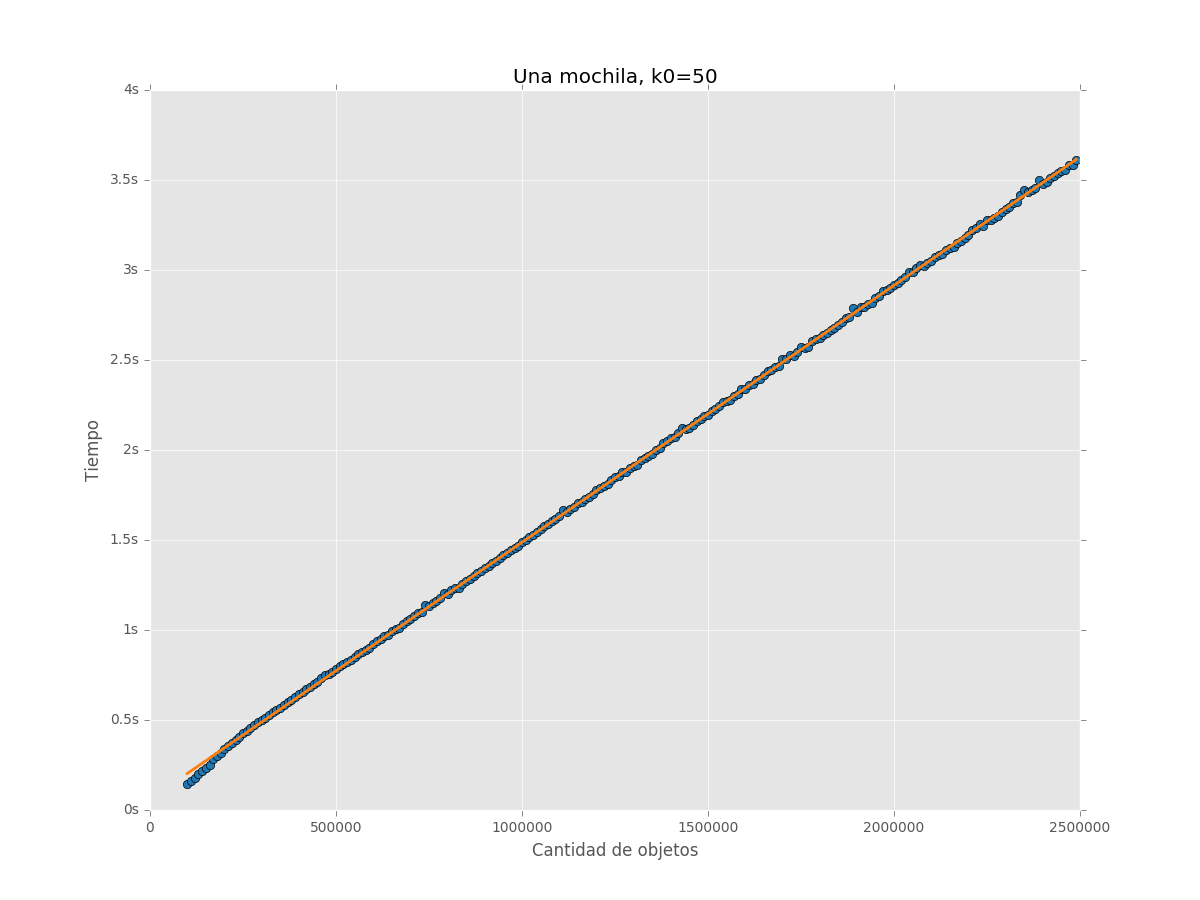
\includegraphics[width=\textwidth]{ej3-c1}
	\end{figure}

\begin{figure}[H]
		\centering
		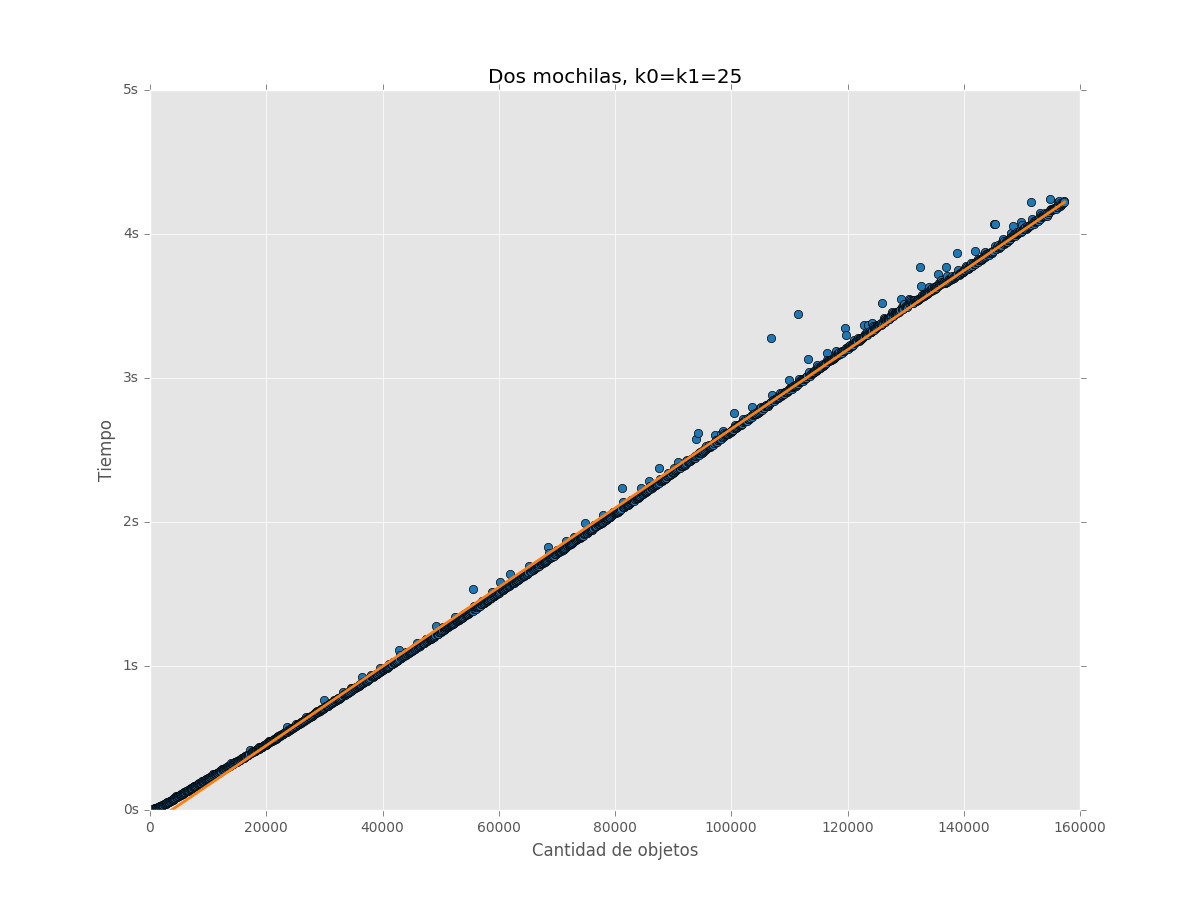
\includegraphics[width=\textwidth]{ej3-c2}
	\end{figure}

\begin{figure}[H]
		\centering
		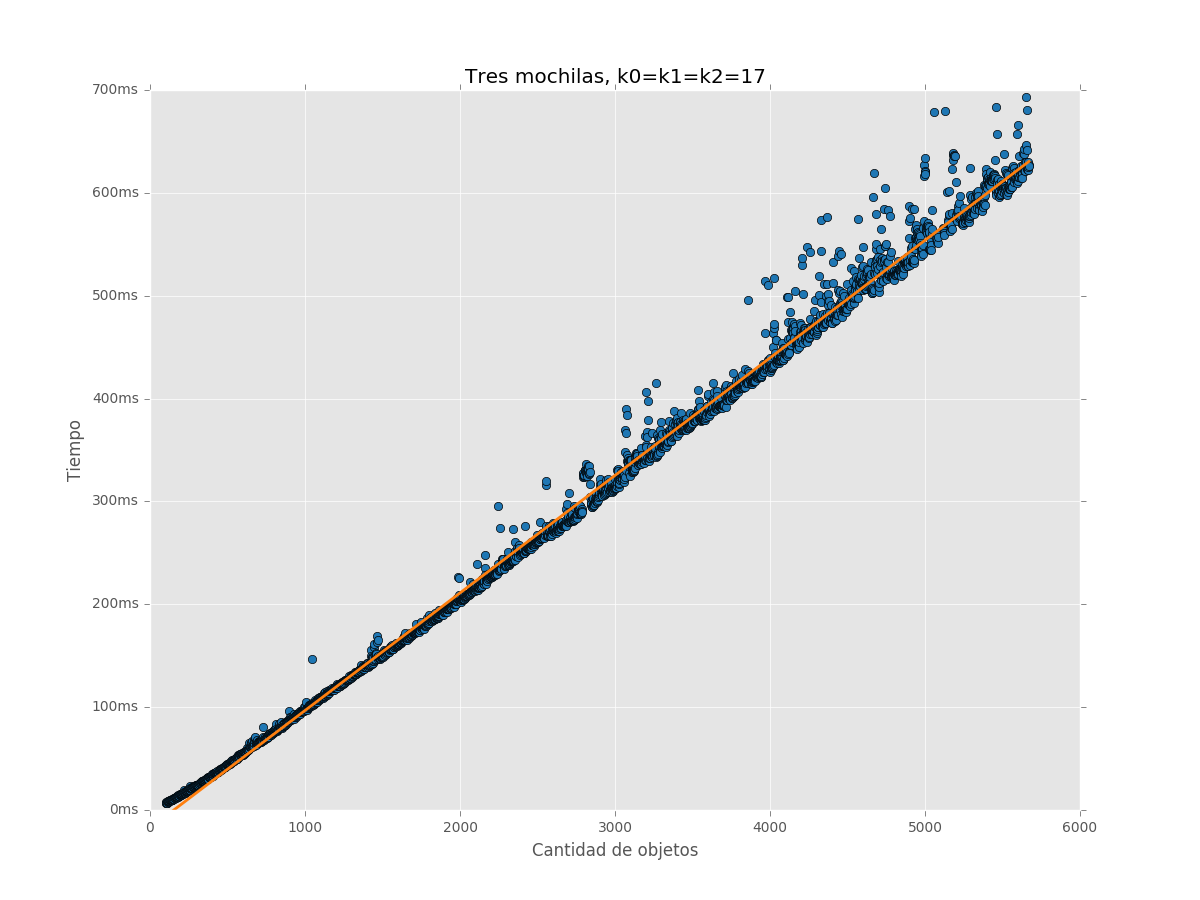
\includegraphics[width=\textwidth]{ej3-c3}
	\end{figure}

Como puede verse, el algoritmo presenta un comportamiento lineal con respecto a la cantidad de objetos, lo cual es entendible ya que si dejásemos fijos los demás parámetros, la complejidad temporal sería $\mathcal{O}(\sum C_i)$. %Por ahí chamuyé re mal acá. No se que más poner D:

\subsubsection{Variando $\prod K_i$}

Dejando fija la cantidad de objetos, se obtuvieron los siguientes resultados de tiempo de ejecución en función de $\prod K_i$ para una, dos y tres mochilas:

\begin{figure}[H]
		\centering
		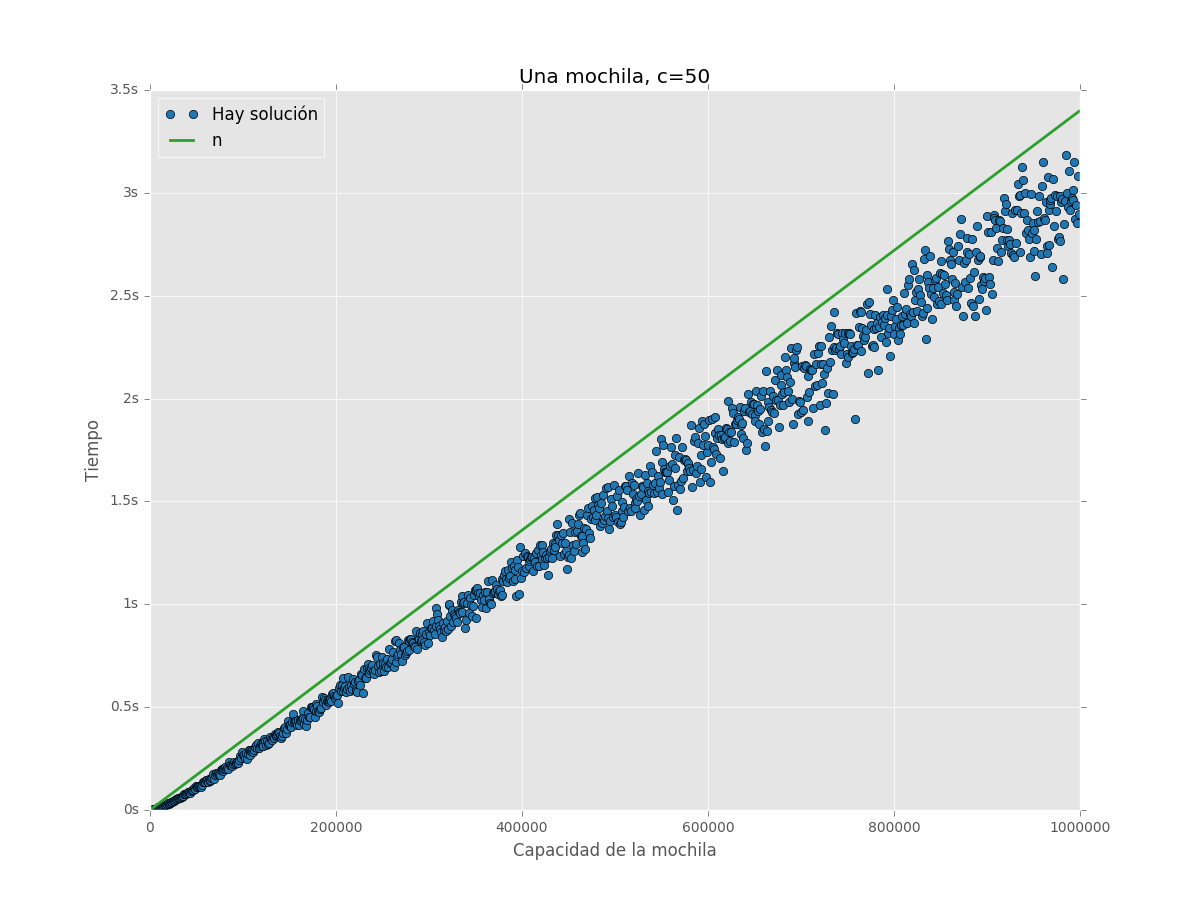
\includegraphics[width=\textwidth]{ej3-k1}
	\end{figure}

\begin{figure}[H]
		\centering
		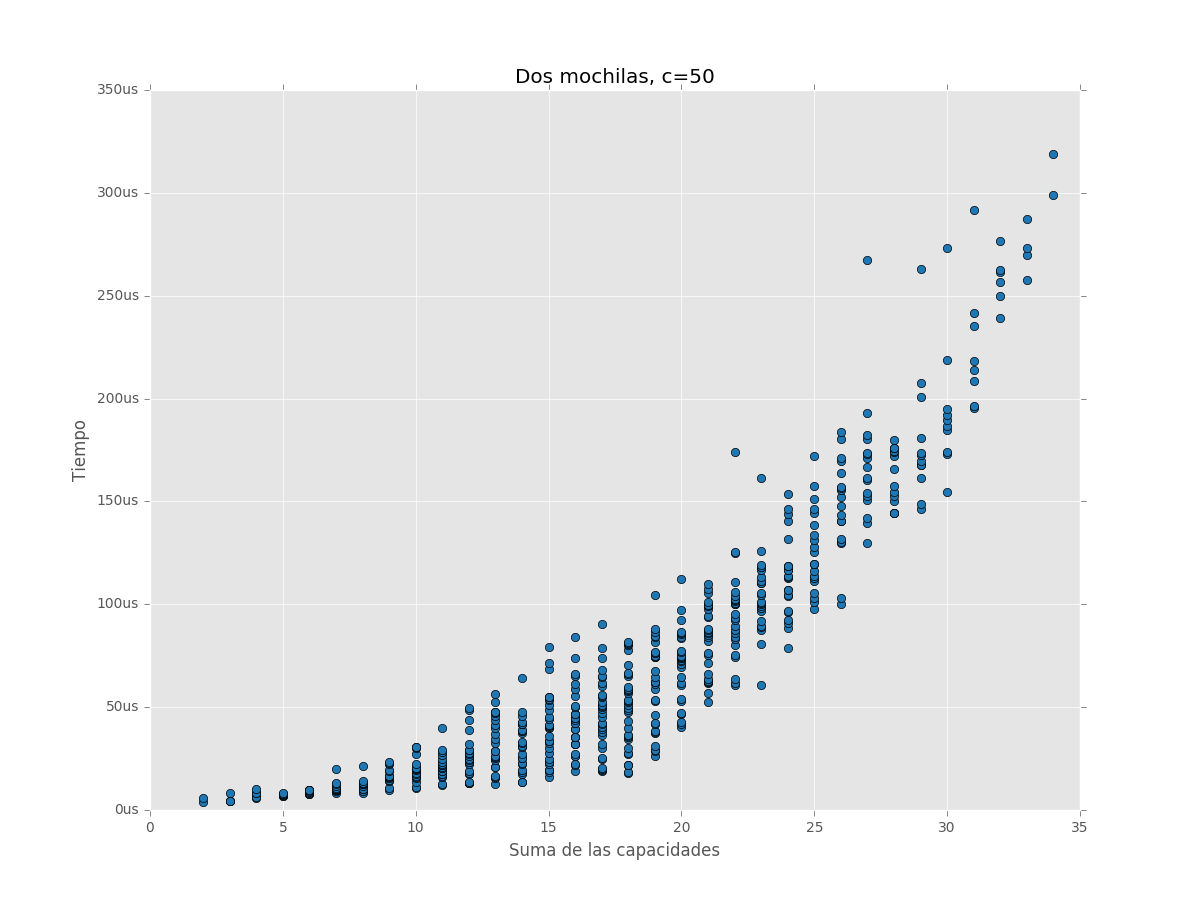
\includegraphics[width=\textwidth]{ej3-k2}
	\end{figure}

\begin{figure}[H]
		\centering
		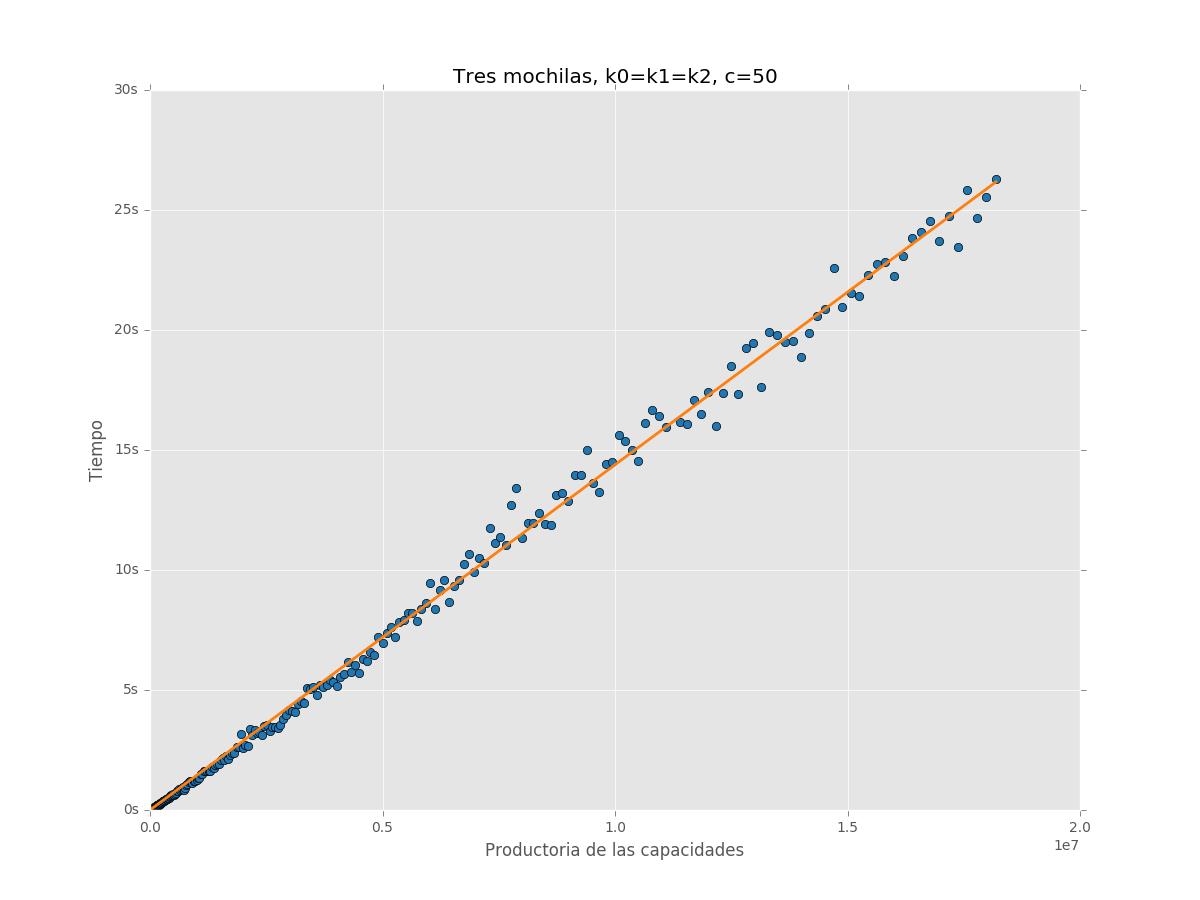
\includegraphics[width=\textwidth]{ej3-k3}
	\end{figure}	

Esto muestra que si se varía la productoria total de las mochilas, el algoritmo vuelve a presentar un comportamiento lineal, lo cual puede explicarse porque dejando fijas todas las demás variables, el algoritmo tendría una complejidad de $\mathcal{O}(\prod K_i)$

Para profundizar más el análisis, se hicieron más experimentos en los que $k_i = k_j$ y se van aumentando de forma lineal todos juntos, de forma tal que $\prod K_i = K_i^M$

\begin{figure}[H]
		\centering
		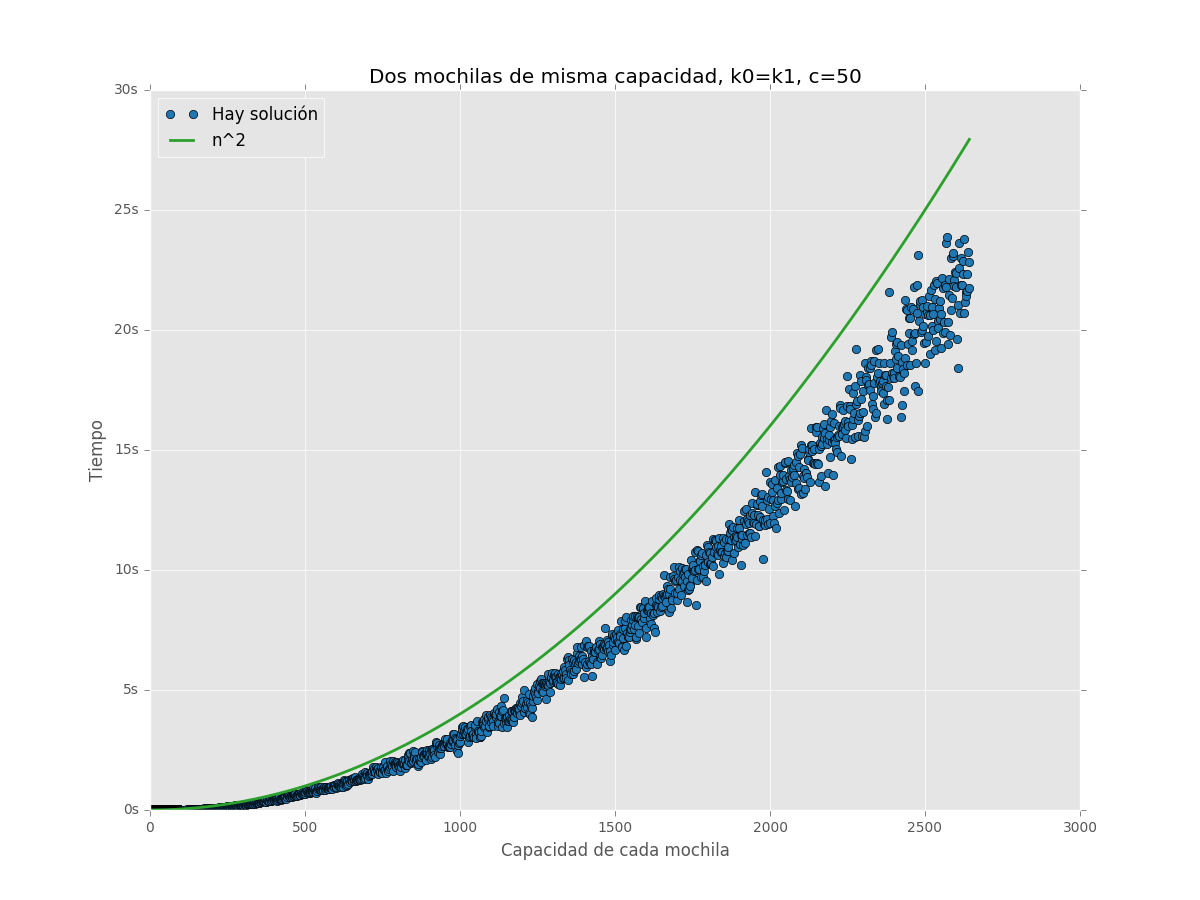
\includegraphics[width=\textwidth]{ej3-k2a}
	\end{figure}	

Aquí se ve que el gráfico presenta un comportamiento cuadrático del algoritmo.

\begin{figure}[H]
		\centering
		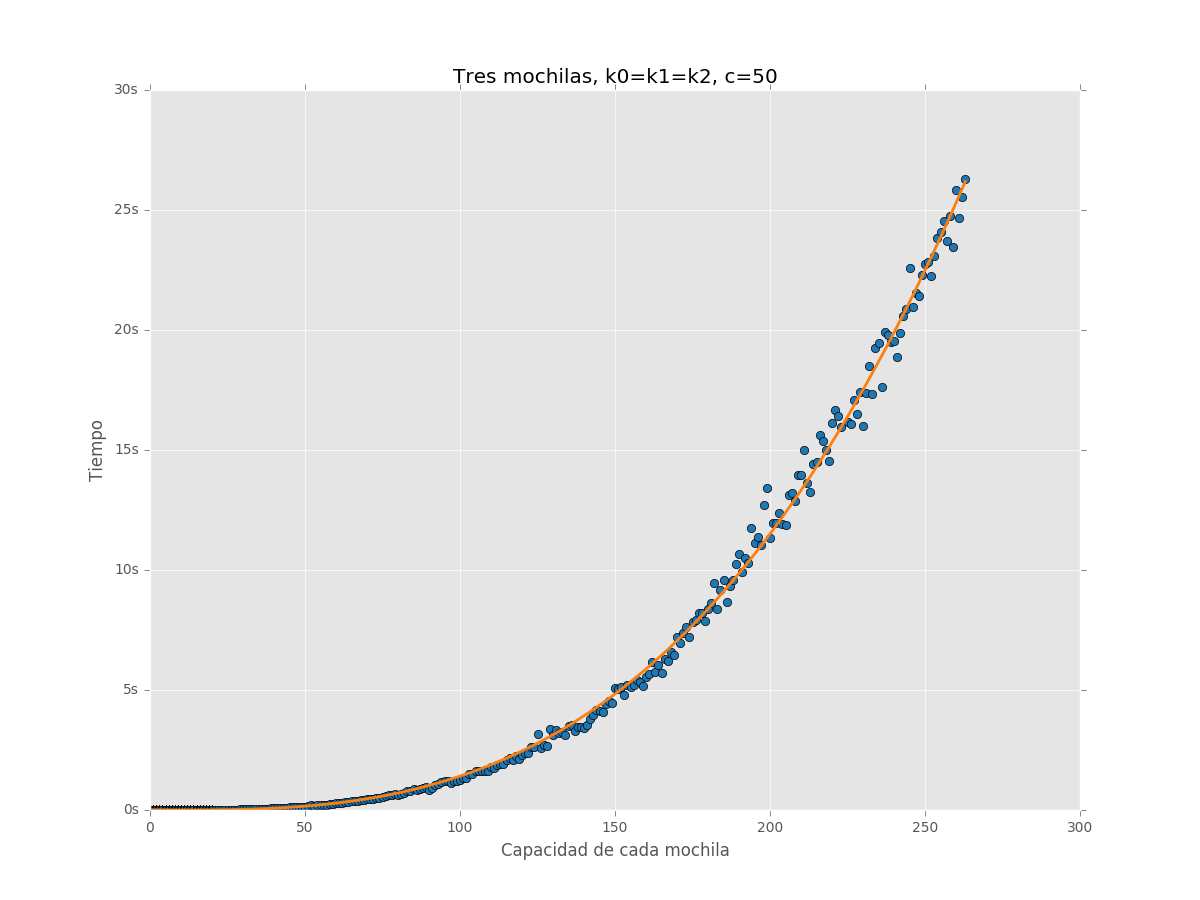
\includegraphics[width=\textwidth]{ej3-k3a}
	\end{figure}	

Y aquí se ve que el gráfico presenta un comportamiento cúbico del algoritmo.

Esto comprueba una vez más las hipótesis de complejidad que fueron presentadas en la sección anterior, ya que evidencia aún más la presencia de la productoria como factor determinante en el tiempo de ejecución.